\section{K-means и EM-алгоритм}
{\it Николай Анохин: <<Самая сложная лекция курса. Если в ней разобраться, то дальше легче будет!>>}

 Сегодня мы попытаемся понять, что средства статистического моделирования и машинного обучения непрерывно связаны. 

\begin{figure}[H]
\centering
    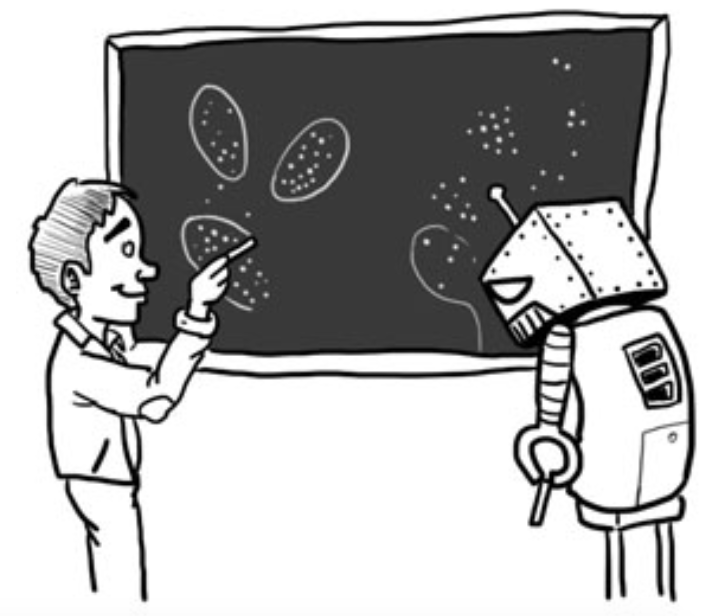
\includegraphics[width=50mm]{images/img1.png}
  %  \caption{Пример кластеризации методом DBSCAN с начальной точкой B1.}
  %   \label{img1}
\end{figure}

\subsection{Задача кластеризации}

На прошлой лекции мы разбирали такие понятия, как {\bf обучение без учителя} и {\bf обучение с учителем.} В первом случае значение целевой функции для объектов из обучающей выборки неизвестно. Поэтому решение таких задач подразумевает исследование <<скрытой структуры>> данных. 

Сегодня мы с Вами рассмотрим {\bf задачу класстеризации}.
\begin{Def}{Задача кластеризации}
"--- задача без учителя, подразумевающая разбиение множества объектов на непересекающиеся подмножества (кластеры) так, чтобы каждый кластер состоял из схожих объектов, а объекты разных кластеров существенно отличались.
\end{Def}


Существенное отличие задачи кластеризации заключается в том, что нам дано {\bf output space} (конечная обучающая выборка объектов), но нет целевой переменной.

%От обучение без учителя в первую отличается тем, что нет значения целевой функции.
Наша задача "--- загруппировать выборку на непересекающиеся подмножества, называемые кластерами, так, чтобы каждый кластер состоял из объектов, близких по метрике. 
Это означает, что всё, что у нас изначально есть "--- это {\it признаковое описание} наших объектов, и нам необходимо выбрать существенные признаки и разбить на группы, то есть кластеризовать, наши объекты.

Большинство алгоритмов подразумевают, что мы знаем, какаое количество кластеров должны получить. Однако на практике чаще ставится задача определить оптимальное число кластеров, с точки зрения того или иного критерия качества кластеризации.\\

{\it Зачем вообще так необходимо заниматься задачей кластеризации?}
\begin{enumerate}
\item Кластеризация позволяет больше узнать о данных (knowledge discovery!);
\item Работать с кластерами удобнее, чем с отдельно взятыми объектами;
\item Кластеризация позволяет конструировать новые признаки.
\end{enumerate}

\subsubsection{Постановка задачи кластеризации}
\begin{Zad} 
Во-первых нам дана обучающая выборка из $N$ объектов, которые мы обозначаем за $x \in {\bf X}$ (trainig data set). 
Необходимо найти модель из семейства параметрических функций вида
\[
H = \left\{h(x,\theta): X \times \Theta \to Y | Y = \{1,\dots,K\}\right\},
\]
ставящую в соответствие произвольному $x \in$ {\bf X} один из $K$ кластеров так, чтобы объекты внутри одного кластера были похожи, а объекты из разных кластеров различались. То есть наша цель выбрать такие параметры $\theta$, которые наилучшим образом отображают действительность.
\end{Zad}

Выше представленная формулировка достаточно обобщённая, попробуем разобраться на более конкретном примере.
\begin{Zad} 
Пусть у нас есть некоторый набор объектов с {\bf двумя свойствами}, по которым можно построить гистограмму. Необходимо построить модель, описывающеую данное распределение. Считаем, что знаем, сколько получается "колоколов" на гистограме, но не знаем описываемые параметры наших объектов.
\end{Zad}

{\bf Пункт 1} Для начала разберём простой случай $K = 1$.% ($K$ "--- количество кластеров) 

\begin{Zam} На самом деле это у нас никакая не задача кластеризация, ибо нет никакой группировки. Но мы рассмотрим принцип максимального правдопадобия и научимся с его помощью находить параметры Гауссовского распределения.
\end{Zam}

Задачу можно переформулировать следующим образом: 
\begin{Zad} \label{K=1} У нас есть ружье, положение которого мы зафиксировали. Мы делаем какое-то количетво выстрелов и считаем, что разброс определяется Гауссовским распределением. Необходимо определить, куда на самом деле смотрит прицел
(т.e. нам даны координаты точек попаданий по мишени из гауссовской пушки, а найти нужно куда смещен прицел).
\end{Zad}
\begin{Zam}
Фишер присвоил имя <<Гауссовскому>> распределению, но сам Гаусс использовал в своих работах с геодезическими нормальное распределение.
\end{Zam}

Выпишем вид нормального (Гауссовского) распределения в матричной форме
\begin{equation}\label{norm}
\NN(x|\mu, {\bf \Sigma}) =  \frac{1}{(2\pi)^{\frac{D}{2}}\cdot |{\bf {\bf \Sigma}}|^{\frac{1}{2}}}
\cdot e^{-\frac{1}{2}(x-\mu)^{T}{\bf {\bf \Sigma}}^{-1}(x-\mu)}
\end{equation}
\[
\mu = \int  x p(x)d x, \qquad {\bf {\bf \Sigma}} = E\left[(x - \mu)( x - \mu)^T \right],
\]
где x "--- <<столбик>> размерности $D$, 
$\mu$ "--- ввектор средних (размерности $D$),
${\bf {\bf \Sigma}}$ "--- матрица ковариаций ($D\times D$), 
а~$D$ "--- плотность распределения.

\begin{Zam} 
%Свойства функции распределения: 
${\bf {\bf \Sigma}}$ "--- симметрическая положительно определенная матрица
\end{Zam}

Формализуем нашу задачу
\[
{\bf X} = \{ x\in R^2\}, \qquad
 p( x) \backsim N\left(x|\mu,{\bf {\bf \Sigma}}\right),\qquad 
 \mu \in R^2,\qquad 
 {\bf {\bf \Sigma}} \in R^{2 \times 2}.
\]
Необходимо найти вектор средних $\mu$ и матрицу ковариации ${\bf {\bf \Sigma}}$.

%Вероятностное распределение непрерыывное, поэтому можно расчитать первый и второй моменты. (они как примеры идут)\\
%Разные виды функкции уровня номрмального распределения,\\ Кружок "--- x = const
%Гаусс распр. Часто встречается в природе. (пр. оценки распредены нормально в классе)
%Центральная предельная теорема: При достаточно общих условиях бесконечная сумма случайных велечин стремится к распредению Гаусса. 
%Пример Биномиальное сумма (распр) стремится к норм распределению
%Плохо D "--- один треугольник вместе с диаганалью $\frac{D(D+1)}{2} + D$ "--- квадратичное количество параметров. (необъодимо переобучение)
%Скажем: давайте будем рассматривать норм распредедения, где ${\bf \Sigma}$  имеет хорошие свойства. (например только $diag({\bf \Sigma}) != 0$, т.е. (c) и (d)).


%Продолжаем решать задачу с Гауссовской пушкой\\
%всего n штук
%x распределеы по нормальному закону. (предпологаем общий вид)
%Representation --- двумерные векторы, распределённые по норм закону


\begin{Zam}
Ранее у нас была следующая формула\\
{ \setlength{\fboxrule}{2pt}
  \setlength{\fboxsep}{8pt}
 \fbox{Learning = Representation + Evaluation + Optimuzation}}
\begin{itemize}
\item Representation -- модель (то, как распределены наши данные). В нашем случае "--- Гауссовское расперделение (иногда бывает линейное)
\item Evaluation --- то, как мы можем проверить наши данные;
\item Optimuzation --- ?
\end{itemize}

{\bf Пример:} Рассмотрим закон Ома $U = I \cdot R$. Изначально мы можем замерить силу тока и напряжение, то есть имеем U и I, а необходимо найти R. Таким образом\\
\begin{itemize}
\item Representation "---  много точек, построили линии;
\item Evaluation "--- наобходимо понять, какая линия самая лучшая на графике (например методом наименьших квадратов);
\item Optimuzation ---?
\end{itemize}
\end{Zam}


\subsection{Принцип максимального правдоподобия}

{\it Пусть у нас есть некий набор данных и гипотиза, как понять --- хорошая ли наша гипотиза или нет?}

Берем гипотизу, вычисляем вероятность, с которой можно пронаблюдать те данные, которые мы видим. Так делаем для всех имеющихся у нас гипотиз (значений параметров). После этого выбраем ту, для которой эта вероятность будет максимальная. То есть та гипотиза, при которой мы имеем больше всего шансов пронаблюдать наши данные и~есть самая лучшая.

\begin{Examp}
Допустим, мы сидим дома, смотрим в окно и видим, что все люди на улице идут с зонтами. В таком случае мы можем сделать собственно предположение, в чём же причина этого.
\begin{itemize}
\item На небе образовалась озоновая дыра, и люди прячуются от вредного излучения под своим зонтом.
\item На улице идет дождь.
\end{itemize}
Конечно, вероятность дождя гораздо выше. По этому по {\bf принципу максимального правдоподобия} на~улице идёт дождь.
\end{Examp}

%Есть у нас набор моделей и мы хотим выбрать ту, которая наилучшим образом соответствует нашим данным.
%Вычисляем вероятность наблюдать наши данные для каждого из значения из параметров, и, соответственно, по значению параметров максимизируем, то есть пытаемся узнать, какие из параметров с максимальной вероятностью породили наши данные.

Теперь давайте формализуем наши рассуждения.
\begin{Def}{Функция правдоподобия}
Пусть дано семейство параметрических моделей $h({\bf x}, \theta)$, где~$\theta$~"---~неизвестные параметры. Предположим, что $p({\bf X}, \theta)$
"--- функция распределения случайной велечены (вероятность), а все наблюдения исходноый выборке независимы и одинаково распределены, тогда {\bf функцией правдопдобия} (likelihood) будет называться их совместная вероятность (плотность), а именно
\[
l({\bf X}|\theta) = \prod\limits_{n=1}^{N} p(x, \theta),
\]
но в нашем курсе функцией правдоподобия мы будем называть её аналог в виде логарифмической~функции~правдоподобия
\[
L({\bf X}|\theta) = \log l = \log \left( \prod\limits_{n=1}^{N} p(x, \theta)\right)
=
\sum\limits_{n = 1}^{N} \log \left( f(x, \theta) \right). 
\] 
\end{Def}

\begin{Def}{Принцип максимального правдоподобия (ML)} %maximum likelihood
"--- это метод оценивания неизвестного параметра путём максимизации функции правдоподобия, который основан на предположении о том, что вся информация о статистической выборке содержится в функции правдоподобия. 
\end{Def}

\subsubsection{Вычисления параметров гауссовской модели}
Вернёмся к нашей задаче~(\ref{K=1}).

\begin{Solution}

Случайные велечены в нашем, в нашем случае "--- координаты точек попаданий по мишени, и все они независимы и одинаково распределены (распределение нормальное). В нашем случае вероятность принимает вид
\[
P(x) = \prod\limits_{n=1}^{N} p({\bf x_n}|\mu,{\bf \Sigma}) \to \max\limits_{\mu, {\bf \Sigma}}.
\]
%смотри формулу (\ref{norm})
Прологорифмируем нашу полную вероятность, а вместо $p(x_n|\mu,{\bf \Sigma})$ подставим нормальное распределение 
\[
 L({\bf X}|\mu,{\bf {\bf \Sigma}}) = \log(P(x)) = \sum\limits_{n = 1}^{N} \log(\NN({\bf x_n}|\mu,{\bf \Sigma}) \to \max\limits_{\mu, {\bf \Sigma}} 
%(с помощью нахождения \mu,{\bf \Sigma})
\]
Для начала честно выпишем, чему равно наше $L({\bf X}|\mu,{\bf {\bf \Sigma}})$ (см.ф-лу.~\ref{norm}).
\[
 L({\bf X}|\mu,{\bf {\bf \Sigma}}) = \sum\limits_{n = 1}^{N} \log(\NN({\bf x_n}|\mu,{\bf \Sigma}) = - \sum\limits_{n=1}^{N}\left(\frac{D}{2} \log 2\pi  +  \frac{1}{2} \log |{\bf {\bf \Sigma}}| + \frac{1}{2} ({\bf x_n} -\mu)^T {\bf {\bf \Sigma}}^{-1} ({\bf x_n} -\mu) \right);
\]
А теперь найдём максимум нашей функции. Для этого продифференциируем её по $\mu$ и приравняем к $0$. Но~перед этим вспомним несколько свойств дифференциирования матриц.
\[
\frac{\partial }{\partial {\bf x}} {\bf x}^T A {\bf x} = (A + A^T)\cdot {\bf x},
\qquad
\frac{\partial }{\partial A} |A| = |A|\cdot \left(A^{-1}\right)^T, 
\qquad
\frac{\partial }{\partial A} {\bf x}^T A{\bf y} = {\bf x}\cdot {\bf y}^T,
\qquad
\frac{\partial }{\partial A} A \cdot B = B^T.
\] 
Поэтому,
\[
\frac{\partial L}{\partial \mu} = \frac{\partial}{\partial \mu}
\left(\frac{1}{2} ({\bf x_n} -\mu)^T {\bf {\bf \Sigma}}^{-1} ({\bf x_n} -\mu) \right) = \dots
\]
Так же вспомним про свойство симметричности матрицы ${\bf \Sigma}$
\[
\dots = 
-\frac{1}{2}\sum\limits_{n = 1}^{N} \underbrace{\left({\bf \Sigma}^{-1} + \left({\bf \Sigma}^{-1} \right)^T \right)}_{2\cdot {\bf \Sigma}^{-1}} \left( {\bf x_n} - \mu \right) 
=
-{\bf \Sigma}^{-1} \cdot \sum\limits_{n = 1}^{N} \left( {\bf x_n} - \mu \right) 
=
 {\bf \Sigma}^{-1} \left(N\cdot \mu - \sum\limits_{n = 1}^{N} {\bf x_n} \right) = 0;
\]
Соответственно,
\[
\sum_{n=1}^{N}  {\bf x_n} = N \cdot \mu \quad \Longrightarrow \quad
 \mu_{ML} = \frac{1}{N} \sum_{n=1}^{N} x_n, 
\]
А теперь аналогично найдём ${\bf \Sigma}_{ML}$, только  искать максимум $L$ будем через параметр ${\bf \Sigma}^{-1}$, то есть
\[
\frac{\partial L}{\partial {\bf \Sigma}^{-1}} = 
 \frac{1}{2} \left(\sum\limits_{n=1}^{N} \frac{\partial}{\partial {\bf \Sigma}^{-1}} \left(\log |{\bf {\bf \Sigma}}|\right) +  \sum\limits_{n=1}^{N}\frac{\partial}{\partial {\bf \Sigma}^{-1}} \left( ({\bf x_n} -\mu)^T {\bf {\bf \Sigma}}^{-1} ({\bf x_n} -\mu) \right) \right) = \dots
 \]
Несложно показать, что в нашем случае 
\[
({\bf x_n} -\mu)^T {\bf {\bf \Sigma}}^{-1} ({\bf x_n} -\mu) = tr\left({\bf {\bf \Sigma}}^{-1} ({\bf x_n} -\mu)({\bf x_n} -\mu)^T\right), 
\]
Тогда
\[
\dots = 
  \frac{1}{2} \left(N \cdot \frac{\partial}{\partial {\bf \Sigma}^{-1}} \left(\log |{\bf {\bf \Sigma}^{-1}}|\right) +  \sum\limits_{n=1}^{N}\frac{\partial}{\partial {\bf \Sigma}^{-1}} tr\left({\bf {\bf \Sigma}}^{-1} ({\bf x_n} -\mu)({\bf x_n} -\mu)^T\right) \right) =
\]
\[
= \frac{1}{2} \left(N \cdot \frac{|{\bf {\bf \Sigma}^{-1}}| \cdot \left(\left( {\bf {\bf \Sigma}^{-1}}\right)^{-1}\right)^T }{|{\bf {\bf \Sigma}^{-1}}|}
+  \sum\limits_{n=1}^{N} \left(({\bf x_n} -\mu)({\bf x_n} -\mu)^T\right)^T \right) =
\]
\[ =
\frac{1}{2} \left(N \cdot {\bf {\bf \Sigma}} + \sum\limits_{n=1}^{N}\left(({\bf x_n} -\mu)^T\right)^T \cdot ({\bf x_n} -\mu)^T \right)= 
\frac{1}{2}\left(N \cdot {\bf {\bf \Sigma}}  + \sum\limits_{n=1}^{N}({\bf x_n} -\mu)({\bf x_n} -\mu)^T \right) = 0
\]
\[
{\bf {\bf \Sigma}_{ML}} = \frac{1}{N} \sum\limits_{n=1}^{N}({\bf x_n} -\mu)({\bf x_n} -\mu)^T
\]
\end{Solution}

\subsubsection{Сложности в работе с принципом правдоподобия}
\begin{enumerate}
\item схлопование компонент;
\item переименование кластеров;
\item невозможно оптимизировать.
\end{enumerate}

\subsubsection{Нахождения параметров смеси нормальных распределений}
{\bf Пункт 2.} А теперь давайте рассмотрим случай, когда наши данные исходят не из одного, а из дувух нормальных распределений ($K = 2$). 

Небольшое предисловие. В америке есть национальный парк, который называется {\it Yellow Stone}, в котором <<типа красиво>>. Там происходят извержения гейзеров, но все проблема в том, что они не регулярны, и поэтому пронаблюдать их сложно. Один из самых известных "--- {\it Old Faithful}. Давайте построим модель, по которой можно будет предсказать время извережения и его длительность.

Была собрана статисктика по извержению гейзеров по следующим параметрам: время извержения и разница во времени между извержениями.
Допустим, мы хотим взять и построить модель на основе наших данных. Наш набор данных двухмерный и очень удобный, мы можем посмтреть, как наша модель работает. Так же у него есть очевидная структура и мы можем сказать, что если мы сделаем всё правильно, то мы что-нибудь да увидим, а именно 2 кластера (как показано на рис.~()).

Как нам к этой задаче приступить?

Рассмотрим суперпозицию 2-ух гауссовских распредений (только мы заведомо не знаем, к которому из них какие точки относятся, т.е. они смогут попасть, как в один так и в другой). То есть у нас имеется двумерная случайная велечина ${\bf z} = (z_1,z_2) \in \R^2$, которая обозначает принадлежность объекта к одному из кластеров, то есть может принимать только два вида: ${\bf z} = (0,1)$ или ${\bf z} = (1,0)$. Принадлежность точки к первому или второму кластеру обозначение следующим образом 
\[
p(z_1 = 1) = \pi_1, \qquad p(z_2 = 1) = \pi_2,
\]
где $p(z)$ --- априорнок распределение на всём векторе 
{\bf z} (распределение 0 и 1). Несложно заметить, что
\begin{equation}\label{apriory}
\sum\limits_{k=1}^K z_k = 1, \qquad
\sum\limits_{k=1}^K \pi_k = 1, \qquad
p(z) = 
 %\begin{cases}
 %\pi_1 \cdot \pi_2, & z_1, z_2 \\
 %\pi_2 & z_2
 %\end{cases} 
 \prod\limits_{k=1}^{K} \pi_k^{z_k} 
\end{equation}
(так же предполагаем, что все $\pi_k$ ненулевые).

Распределение {\bf X} для каждого из K кластеров будем считать нормальным (\ref{norm}) (каждому кластеру соответствует свой вектор средних и своя матрица ковариации), тогда для $\forall x \in {\bf X}$
\[
p(x|z_k) = N (x|\mu_k,{\bf \Sigma}_k) 
\quad \Longrightarrow \quad
p(x|{\bf z}) = \prod\limits_{k=1}^K \left(\NN(x|\mu_k,{\bf \Sigma}_k)\right)^{z_k}
\]
%А значит смесь нормальных распределений будет представима в виде
%\[
%p({\bf X} , {\bf z}) = \prod\limits_k [ \pi_k \NN(x|\mu,{\bf \Sigma}_k)]^{z_k},
%\]
%а функция правдоподобия всей системы
Будем опускать потихоньку параметры модели и найдём распределение {\bf X}
\[
p(x) = p(x|\pi, \mu,{\bf \Sigma}) = \underbrace{p(x|{\bf z})\cdot p({\bf z})}_{\text{по формуле полной вероятности}} =  
%\sum\limits_{k=1}^K \prod\limits_j \left(\NN(x|\mu_j,{\bf \Sigma}_j) \cdot \pi_j \right)^{z_j} =
\sum\limits_{k=1}^{K} \pi_k \NN(x|\mu_k,{\bf \Sigma}_k).
\]
На самом деле это то, что мы и ожидали увидеть, а именно смесь Гауссовских распределений, которые соответствуют априорной вероятности появления $x$ в неком кластере.

Чтобы нам было проще жить, введём следующую велечину
\[
\gamma(z_k) = p(z_k = 1| x) = \underbrace{\frac{ p(z_k = 1)\cdot p(x|z_k=1)}{p(x)}}_{\text{по формуле Байеса}}
 = \frac{ \pi_k \NN(x|\mu_k,{\bf \Sigma}_k)}{\sum\limits_{j=1}^K \pi_j \NN(x|\mu_j,{\bf \Sigma}_j)}
\]
 
Раньше, до того, как мы начали иметь дело с нашими данными, у нас было единственное предположение~(\ref{apriory})~"---~априорное распределение.
А $\gamma$ "--- апостериорное распределение, то есть вероятность того, что мы попали в кластер под номером $k$, если пронаблюдали $x$.


Теперь мы уже готовы применять принцип максимального правдоподобия. Поэтому выпишем функцию максимального правдоподобия и сразу же возьмём логорифм.
\[
p({\bf X}|\pi,\mu,{\bf \Sigma}) = \underbrace{\prod\limits_{n=1}^{N} p(x_n|\pi,\mu,{\bf \Sigma})}_{\text{произведение превратится в сумму}}\quad
\Longrightarrow \qquad
L({\bf X}|\pi,\mu,{\bf \Sigma}) = \log \left (p({\bf X}|\pi,\mu,{\bf \Sigma})\right) =
\]
\[
= \sum_{n=1}^K \log \sum\limits_{k=1}^K \pi_k \NN(x_n|\mu_k,{\bf \Sigma}_k) 
\quad \to\quad max (\pi,\mu,{\bf \Sigma}).
\]
Далее продифференциируем функцию правдоподобия по каждому из параметров, возьмём точки, где функция обращается в ноль, исследуем минимум это или максимум и всё здорово. Есть только одна проблема: эту функцию вполне можно продифференциировать, но найти решение полученных уравнений аналитически будет невозможно, в отличии от одномерного случая.

Для начала продифференциируем по $\mu$
\[
\frac{\partial L}{\partial \mu_k} =  \sum_{n=1}^N  \underbrace{\frac{ \pi_k \NN(x_n|\mu_k,{\bf \Sigma}_k)}{ \sum\limits_{j=1}^K  \pi_j \NN(x_n|\mu_j,{\bf \Sigma}_j)}}_{\gamma_{z_{nk}}} \cdot {{\bf \Sigma}^{-1} (x_n - \mu_k)} 
= \sum_{n = 1}^N \gamma_{z_{nk}}(x_n - \mu_k) = 0;
\]
\[
\mu_k = \frac{\sum\limits_{n=1}^N \gamma(z_{nk})x_n}{\sum\limits_{n=1}^{N}\gamma(z_{nk})} = \frac{1}{N_k}\sum\limits_{n=1}^N \gamma(z_{nk})x_n,
\]
где $N_k$ "--- эффективное количество элементов в кластере.
Аналагично получим
\[
{\bf \Sigma}_k = \frac{1}{N_k} \sum_{n=1}^{N} \gamma(z_{nk}) (x_n - \mu_k)^T(x_n-\mu_k), \qquad \pi_k = \frac{N_k}{N}.
\]
Наконец, кажется всё здорово и задачу мы вроде бы решили, но есть одна проблема: $\gamma$ зависит от всего, то есть от $\mu$, ${\bf \Sigma}$ и $K$. Нам удалось получить какие-то выражения, но они не представляют из себя решения, ибо вычислить мы ничего не можем. Однако вычислить мы всё-таки что-то хотим, для этого воспользуемся EM-алгоритмом.

\subsection{EM-алгоритм}
EM-алгоритм (Expectation Maximization)
 "--- это, то что сегодня является центром нашей лекции.
%Рассмотрим EM-алгоритм (Expectation Maximization)
Идейно алгоритм очень простой. На каждой итерации последовательно выполняется два шага. 

На первом шаге ({\bf E}) мы высчитываем наши $\gamma$, то есть считаем, что мы как бы знаем $\mu, {\bf \Sigma}, \pi$, и расскидываем наши объекты по кластерам.

На втором шаге({\bf M}) мы используем вычисленные $\gamma$ и на их основании мы высчитываем новые значения параметров.

Хорошее тут то, что процедура гарантрированно сходится.
Можно доказать, что на каждом из шагов likelihood никогда не убывает: он может оставаться таким же или возрастать. Рано или поздно мы упрёмся в экстремум, то есть локальный максимум.
\begin{Zam}
В нашем случае очень важно <<локальный>>, ибо EM не гарантирует глобальной максимизации. То есть, когда мы что-то нашли мы не можем гарантировать, что наше решение оптимально глобально (только локально). Однако с этим можно бороться.
\end{Zam} 

Иллюстрацию работы алгоритма можно посмотреть на рис.~(\ref{EM})

\begin{figure}[H]
\centering
    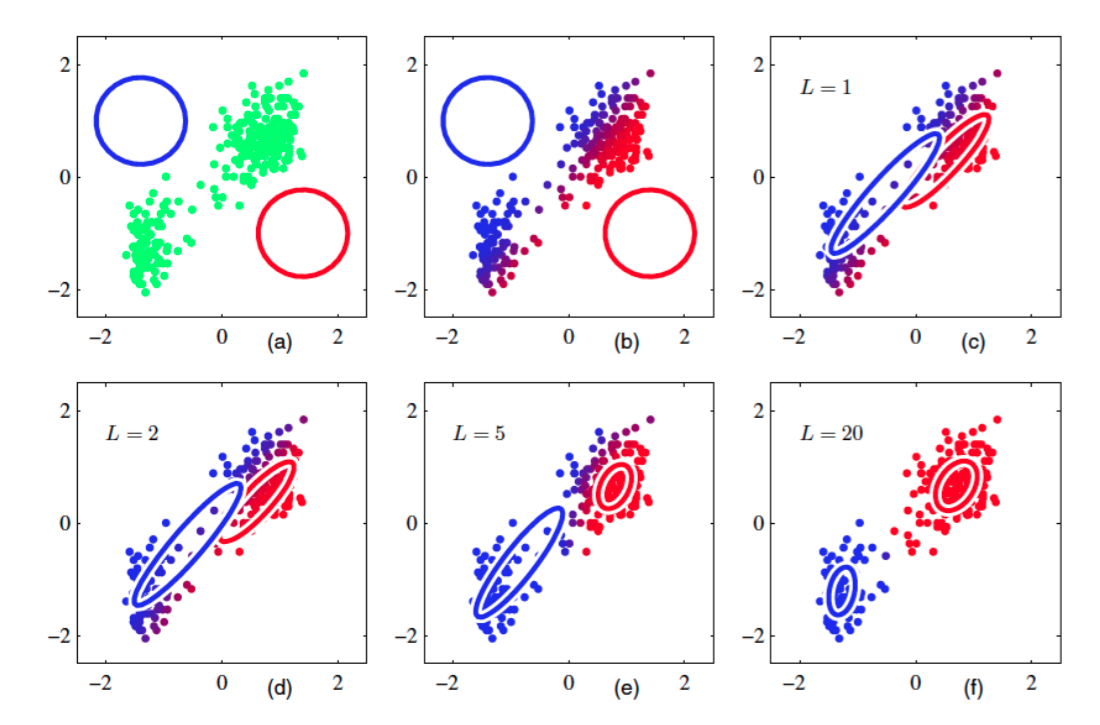
\includegraphics[width=100mm]{images/EM.png}
    \caption{Пример работы EM алгоритма.}
    \label{EM}
\end{figure}

Оказывается, что алгоритм EM можно обобщить на произвольных случай неизвестных переменных,
На шаге E мы вычисляем распределение латентных (скрытых) переменных $p \left({\bf z| X}, \theta^{old}\right)$, при учёте, что нам даны <<старые>> параметры модели (начинаем со случайных). Этому распределению соответствуют наши $\gamma$, которые мы уже ранее обсуждали.

На шаге M мы высчитываем 
$\theta^{new} = \mathrm{arg} \max\limits_{\theta} Q(\theta,\theta^{old})$, через
математическое ожидание по {\bf z} логарифма совместного распредления {\bf x} и {\bf z}. 
\[
Q(\theta,\theta^{old}) =
E_{\bf z} \left[\ln p({\bf X, z}|\mu,{\bf \Sigma}, \pi)\right] = \sum\limits_{{\bf z}} p({\bf z|X},\mu,{\bf \Sigma}, \pi) \ln p({\bf X, z}|\mu,{\bf \Sigma}, \pi) 
\]
Как раньше это всё происходит до сходимости.


Так жу в данном случае есть способ улучшить наш алгоритм, введя априорное распределение $p(\theta)$ с помощи формулы Байеса.
%$Е_z$ "--- ожидание по вероятности алгоритма совместного распределения. С точность д константы апроксимизирует.

%MVN --- многомерное гауссовское распределение

\subsection{K-means}

Алгоритм представляет собой версию EM-алгоритма, применяемого также для разделения смеси гауссиан. Он разбивает множество элементов векторного пространства на заранее известное число кластеров k.

Основная {\bf идея} алгоритма заключается в том, что на каждой итерации перевычисляется центр масс для каждого кластера, полученного на предыдущем шаге, затем векторы разбиваются на кластеры вновь в соответствии с тем, какой из новых центров оказался ближе по выбранной метрике.

Алгоритм завершается, когда на какой-то итерации не происходит изменения центра масс кластеров. Это происходит за конечное число итераций, так как количество возможных разбиений конечного множества конечно, а на каждом шаге суммарное квадратичное отклонение не увеличивается, поэтому зацикливание невозможно.

%\begin{Zam} Функция правдоподобия не обязана быть выпуклой. Можно упиреться в локальный максимум, не добравшись до глобального. \end{Zam}

А теперь давайте немного формализуем наши рассуждения.

Пусть матрицы ковариации все одинаковые, а ещё и круглые, т.е. ${\bf \Sigma}_k = \e \cdot Id$. $Det({\bf \Sigma}_k) = \e$, тогда 
\[
p(x|\mu_k, {\bf {\bf \Sigma}_k}) = \NN(x|\mu_k,{\bf \Sigma}_k) = \frac{1}{\sqrt{2\pi \e}} e^{-\frac{1}{2\e} ||x - \mu_k||^2}
\]

Рассмотрим предельный переход $\e \to 0$
\[
\gamma_{nk}  = \frac{ \pi_k \NN(x|\mu_k,{\bf \Sigma}_k)}{\sum\limits_{j=1}^K \pi_j \NN(x|\mu_j,{\bf \Sigma}_j)}
 = \frac{ \pi_k e^{-\frac{1}{2\e} ||x_n - \mu_k||^2}}{\sum\limits_{j=1}^K \pi_j e^{-\frac{1}{2\e} ||x_n - \mu_j||^2}} 
\quad \to \quad
r_{nk} = 
\begin{cases}
1, \quad \text{для } k = \mathrm{arg}\min\limits_{j} || x_n - \mu_k||;\\
0, \quad \text{иначе.}
\end{cases}
\]
Таким образом $\gamma$  "--- это просто функции вхождения $n$-го элемента в $k$-й кластер. Она будет стремиться к 1 для ближайшего кластера, для остальных к 0.
Функция правдоподобия принимает вид
\[
E_{\bf z} \left[\ln p({\bf X, z}|\mu,{\bf \Sigma}, \pi)\right] 
%= \sum\limits_{{\bf z}} p({\bf z|X},\mu,{\bf \Sigma}, \pi) \ln p({\bf X, z}|\mu,{\bf \Sigma}, \pi) 
\to -\sum\limits_{n=1}^N\sum\limits_{k=1}^K r_{nk} ||x_n - \mu_k||^2 + \mathrm{const}, 
\]
\[
\mu_k = \frac{\sum\limits_{n=1}^N r_{nk} x_n}{\sum\limits_{n=1}^N r_{nk}}.
\]


\begin{Zam}
Не сложно заметить, что в знаменателе последней формулы стоит просто количество элементов в кластере.
\end{Zam}

%Помогает оптимизировать функции правдоподобия, когда есть скрытые переменные.


%$\gamma (z_{nk})$ .
%То есть имеем жесткую принадлежность к кластеру
%вводим величину $r_{nk} = 1$, если k --- ближайший к n кластер, иначе $r_{nk} = 0$.

%от внутренней суммы останется тлько плижайшей компонент (6ая строчка)
%Этот переход называется переход от EM-алг к  K-means

%минус K-means --- локальная кластеризация

Таким образом, используя идею EM-алгоритма, мы перешли к одному из замых известных алгоритмов кластеризации k-means. Получается, между вероятностной моделью и моделью машинного обучения есть связь: алгоритм k-means по сути базируется на модели смеси гауссовских распределений.

\subsubsection{Алгоритм работы программы}
Рассмотрим алгоритм в виде псевдокода на языке $Python$:
\begin{lstlisting}
function kmeans(X, K):
    initialize N # number of objects
    initialize Mu = (mu_1 ... mu_K) # random centroids
    do:
    # E step
        for k in 1..K:
            for x in 1..N:
                compute r_nk # Cluster assignment
    # M step
        for k in 1..K:
            recompute mu_k # Update centroids
    until Mu converged
    J = loss(X, Mu)
    return Mu, J
\end{lstlisting}

Несложно заметить, что сложность данного алгоритма равна $O(NK)$. Так же на рисунке~(\ref{k-means}) представлен пример реализции данного метода.

\begin{figure}[H]
\centering
    \includegraphics[width=100mm]{images/KM.png}
    \caption{Пример работы алгоритма k-means.}
    \label{k-means}
\end{figure}


\subsubsection{Проблемы}
\begin{enumerate}
\item Оптимизация, как и в случае с EM, является локальной.\\
Для решения этой проблемы есть такая традиция запускать k-means много раз, случайным образом выбирая начальные центры кластеров. В качестве лучшего выбираем тот, где значение функции потерь $J$ минимальна. Практика показывает, что количество перезапуска этого алгоритма должна начинаться примерно от 1000 раз.
\item Данных слишком много.\\
Решение: Если не можем загрузить все данные, то можно выбирать какое-то подмножество и на его основе построить центроиды. После этого разбить всё множество на соответствующие кластеры с уже имеющимися центрами. (данная модификация алгоритма называется {\it mini-batch k-means})
\item Признаки не числовые\\
Решение: x = \{набор различных признаков объекта\}\\ 
В качестве центройдов -- не целое значение, а какого-то типичного представителя и с ним сравнивать. Функция сравнения "--- $d(x_i,x_j)$ "--- расстояние до центра (или ещё какого-то параметра).\\
% Например желтый треугольник и красный круг 1 +1\\
% желтый треугольник и желтый круг 0 + 1\\
% расстояние -- 0, если совпали, 1 если нет.
\end{enumerate}

\subsubsection{Критерий качества}
\[
{\ol J} = \sum\limits_{n=1}^N \sum\limits_{k=1}^k r_{nk} d(x_n,\mu_k),
\]
где $d(x_n,\mu_k)$ "--- функция расстояния, 
$\mu_k$ "--- один из объектов кластера.

Таким образом, качество работы алгоритма зависит от выбранной функции растояния между объектами.
\begin{Zam}
Если с помощью нашей метрики мы не можем найти  центроид кластера, то выбирается один из обучающих объектов, который лежит далеко от границы кластера, в виде типичного представитель. Такой представитель называется medoid, а алгоритм соответственно будет иметь новое название $k-medoids$.
\end{Zam}

\subsubsection{Оптимизация (k-means++)}
(Из Википедии)

Данный алгоритм оптимизирует способ нахождения начальных центроид наших кластеров.
\begin{enumerate}
\item Выбрать первый центроид случайным образом (среди всех точек)
\item Для каждой точки найти значение квадрата расстояния до ближайшего центроида (из тех, которые уже выбраны) $dx^2$
\item Выбрать из этих точек следующий центроид так, чтобы вероятность выбора точки была пропорциональна вычисленному для неё квадрату расстояния\\
Это можно сделать следующим образом. На шаге 2 нужно параллельно с расчётом $dx^2$ подсчитывать сумму $Sum(dx^2)$. После накопления суммы найти значение $Rnd = random(0.0,1.0) \cdot Sum$. $Rnd$ случайным образом укажет на число из интервала $[0; Sum)$, и нам остаётся только определить, какой точке это соответствует. Для этого нужно снова начать подсчитывать сумму $S(dx^2)$ до тех пор, пока сумма не превысит Rnd. Как только это случится, суммирование останавливается, и мы можем взять текущую точку в качестве центроида.\\
При выборе каждого следующего центроида специально следить за тем, чтобы он не совпал с одной из уже выбранных в качестве центроидов точек, не нужно, так как вероятность повторного выбора некоторой точки равна 0.
\item Повторять шаги 2 и 3 до тех пор, пока не будут найдены все необходимые центроиды.
Далее выполняется основной алгоритм k-means.
\end{enumerate}
%k-means++ --- берём один центр рендомно, а другие максимально далеко от первого.

%онлайн, ?

%слайд 30 --- $J$ --- инерция (? или $m_k$) взяли 2 разные нормы.

%По теории всё.

%\subsection{Практика.}

%Задача классификации пользователей сети twitter\\
%nikname\\
%location\\
%registration date\\
%inclass.cagle.com
%2000 пользователей надо разметить

%ля каждого пользователя необходимо собрать данные
%ознакомиться с панда
%с помощью обертки  скачать данные пользователя
%и геолокации

%зарегестрироваться на cagle и отписать свой id в топике, чтобы смогли меня туда допустить

%необходимо отобрать: страну, координаты, 

%графики:
%\begin{enumerate}
%\item Появление аккаунтов, в зависимости от времени
%\item распределение пользователей по карте мира
%\end{enumerate}

%сохранить таблицу с признаками пользователя
%за 2 функции баллы, за улучшения графика --- бонус

%deadline --- понедельник 6 утра

%проект --- классификация пользователей твиттера
%пробная/тестовая выборки.
%кто лучше предскажет -- тот получит макс балл.
%нужно догадаться, какяа категорию. 